\documentclass{beamer}
\usetheme{metropolis}

\usepackage[T1]{fontenc}
\usepackage[type1]{libertine}
\renewcommand{\ttdefault}{cmtt}
\usepackage[font=scriptsize]{caption}
\setbeamerfont{footnote}{size=\scriptsize}

\title{CDP2 Post-processing Documentation}
\subtitle{A Quick Overview}
\date{\today}

\begin{document}

\frame{\titlepage}

\begin{frame}
    \frametitle{Introduction}
    The following document describes the post-processing steps required to produce a sensible dataset from noisy observations from CDP2. Due to various aspects of the detector, post-processing steps are necessary to detect outliers and reduce noise.
\end{frame}

\begin{frame}
    \frametitle{Changes to filtering}
    Thanks to the outlier detection using DSM (see slides 4 and 5), pre-processing filters can now be more lenient.

    Previously, data points had to meet the following criteria:

    \begin{itemize}
        \item DT Bandwidth < 12
        \item DSM (dump spot monitor) > 1 V
        \item ATT (average transit time) < 100 $\mu$s\footnotemark[1]
    \end{itemize}

    which have now been simplified to:

    \begin{itemize}
        \item DSM > 0.6 V
        \item 0.5 $\mu$s < ATT < 160 $\mu$s.
    \end{itemize}

    \footnotetext[1]{This value was initially obtained from PADS manual}
\end{frame}

\begin{frame}
    \frametitle{Check Dump Spot Monitor (DSM)}
    Here is an except from the PADS Overview manual:

    \begin{quotation}
        \small{A channel indicating the amount of focused, unobstructed laser light collected in the dump spot monitor. This channel can indicate overall system health. If the monitor reading goes down when there are no particles present, there may be a problem. (When particles are present, the laser light scatters, which reduces the focused light collected in the dump spot.) It is important to track the trend over a long period of time, for instance over several months, as this channel can change slowly. Overheated lasers or probe windows blocked by fog and/or ice could cause the laser monitor reading to go down even though no particles are present.}
    \end{quotation}
\end{frame}

\begin{frame}
    \frametitle{Check Dump Spot Monitor (DSM)}
    Depending on the status of the sensor, one may need to filter out non-spontaneous\footnotemark[1] drops in DSM.

    \begin{figure}
        \centering
        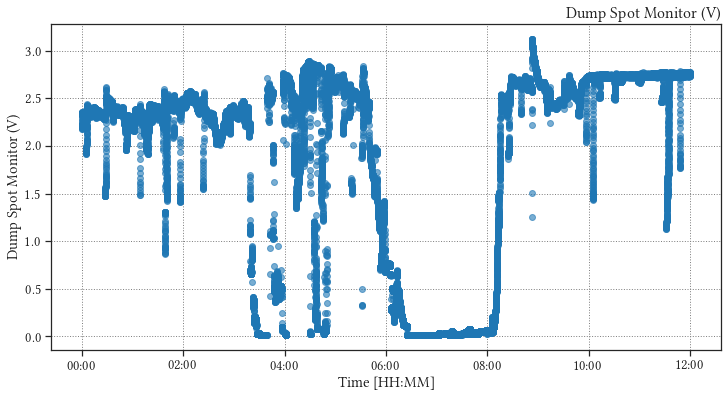
\includegraphics[width=0.7\textwidth]{img/dsm.png}
        \caption{Daily time-series of DSM [V] on June 26th, 2020}
    \end{figure}

    \footnotetext[1]{Sudden, short-term drops in DSM due to blockage are expected, but combined with a long-term degradation of the sensor, the actual behaviour tends to be erratic.}
\end{frame}

\begin{frame}
    \frametitle{Outlier detection with DSM}
    One can further filter out outliers by looking at the changes in DSM. The goal is to detect spontaneous drops in DSM and flag the data points. In order to do so, one can smooth the DSM time-series (using Gaussian convolution, explained later) and find the temporal gradient
    \begin{equation*}
        \partial_t \, \mathrm{DSM} = \frac{\partial}{\partial t} \, \mathrm{DSM}
    \end{equation*}
    which has units of V/s.

    The DSM time-series tends to be quite noisy, so smoothing is necessary for the sake of outlier detection.
\end{frame}

\begin{frame}
    \frametitle{Outlier detection with DSM}
    Then filter out data where $| \partial_t \, \mathrm{DSM} | > 1.5 \times 10^{-4} \, \mathrm{V/s}$\footnotemark[1] (red line).

    \begin{figure}
        \centering
        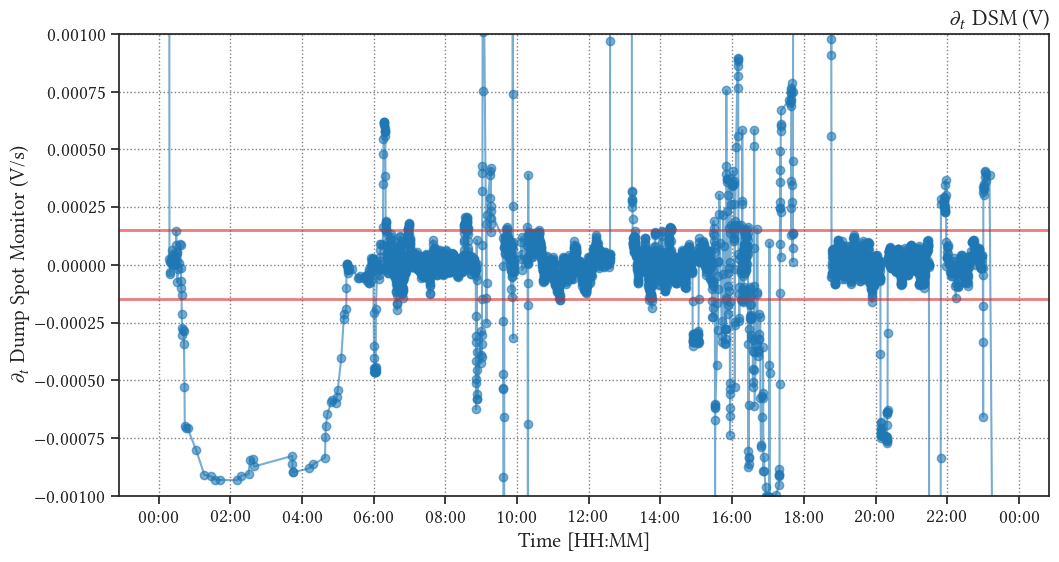
\includegraphics[width=0.7\textwidth]{img/dsm_dt.png}
        \caption{Daily time-series of $\partial_t$ DSM [V] on June 26th, 2020}
    \end{figure}

    \footnotetext[1]{This threshold has been chosen arbitrarily by trial and error, but seems to work well.}
\end{frame}

\begin{frame}
    \frametitle{Notes on Outlier detection}
    The gradient-based outlier detection allows us to filter out outliers in the time-series data by identifying unrealistic peaks in the observed signals.


    This is especially useful since the laser in the particle detector tends to degrade over time --- and because of that, mean DSM decreases, which makes it difficult to separate outliers from normal data (but with DSM < 1 V). Once the outliers can be filtered from the time-series, we can then safely filter unreliable data, which is done by filtering out signals with DSM < 0.6 V.
\end{frame}

\begin{frame}
    \frametitle{Adjust with True PAS}
    Because of the discrepancy between the default passing air speed (PAS) and the actual speed of the particles, one needs to estimate the latter based on average transit time:
    \begin{align*}
         & \mathrm{PAS}_\mathrm{LM} / \mathrm{PAS}_\mathrm{True}                                   \\
         & \approx \mathrm{PAS}_\mathrm{LM} / (150 \, [\mu \mathrm{m}] / \tau \, [\mu \mathrm{s}])
    \end{align*}
    where $\tau$ stands for the average transit time measured by CDP2.\\~\

    Multiply all flux-based measurements (e.g. LWC and NC) by the adjustment factor given above.
\end{frame}

\begin{frame}
    \frametitle{Adjust with True PAS}
    The following shows the effect of using the true speed of the measured particles according to CDP2.

    \begin{figure}
        \centering
        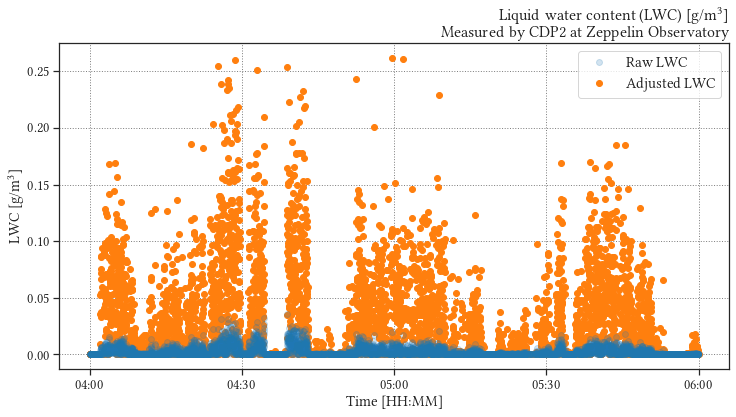
\includegraphics[width=0.7\textwidth]{img/pas.png}
        \caption{Daily time-series of LWC [g/m$^3$] on June 26th, 2020}
    \end{figure}
\end{frame}

\begin{frame}
    \frametitle{Gassuain Smoothing}
    The raw time-series directly from CDP2 tends to be very noisy. To obtain a more useful (and less error-prone) time-series, one can use the Gaussian kernel:
    \begin{equation*}
        K_\mathrm{Gauss} = \frac{1}{\sigma \sqrt{2 \pi}} \mathrm{e}^{-\frac{x^2}{2 \sigma^2}}
    \end{equation*}
    where $\sigma$ defines the \emph{width} of the kernel. Theoretically, this value represents our prior belief about the uncertainty involved in the observations. We will be using $\sigma = 5$ minutes, since we believe that the flux values do not change rapidly.
\end{frame}

\begin{frame}
    \frametitle{Gassuain Smoothing}
    Given the Gaussian kernel $K_\mathrm{Gauss}$, we can calculate the convolution of the time-series $f(t)$ (LWC in this case) and the Gaussian kernel. That is,
    \begin{equation}
        (f * K_\mathrm{Gauss})(t) \triangleq \int_0^t f(\tau) K_\mathrm{Gauss}(t - \tau) \,\mathrm{d} \tau
    \end{equation}
    which yields a smooth, noise-free time-series.
\end{frame}

\begin{frame}
    \frametitle{Gassuain Smoothing}
    \begin{figure}
        \centering
        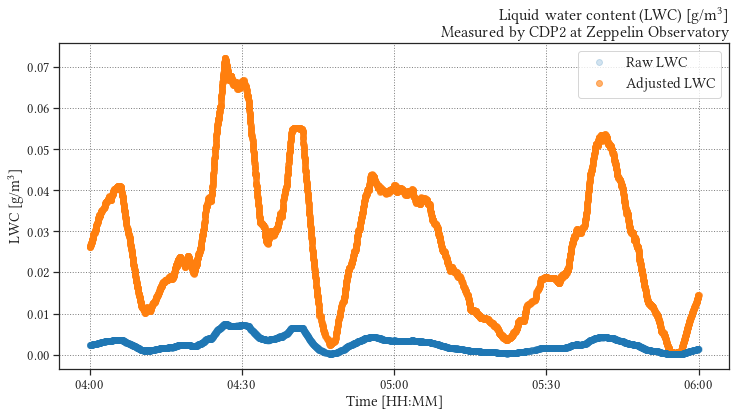
\includegraphics[width=0.7\textwidth]{img/conv.png}
        \caption{Daily time-series of LWC [g/m$^3$] on June 26th, 2020}
    \end{figure}
\end{frame}

\begin{frame}
    \frametitle{Re-sampling with Sparse GP Model}
    Here is a result of temporal re-sampling using GP regression:

    \begin{figure}
        \centering
        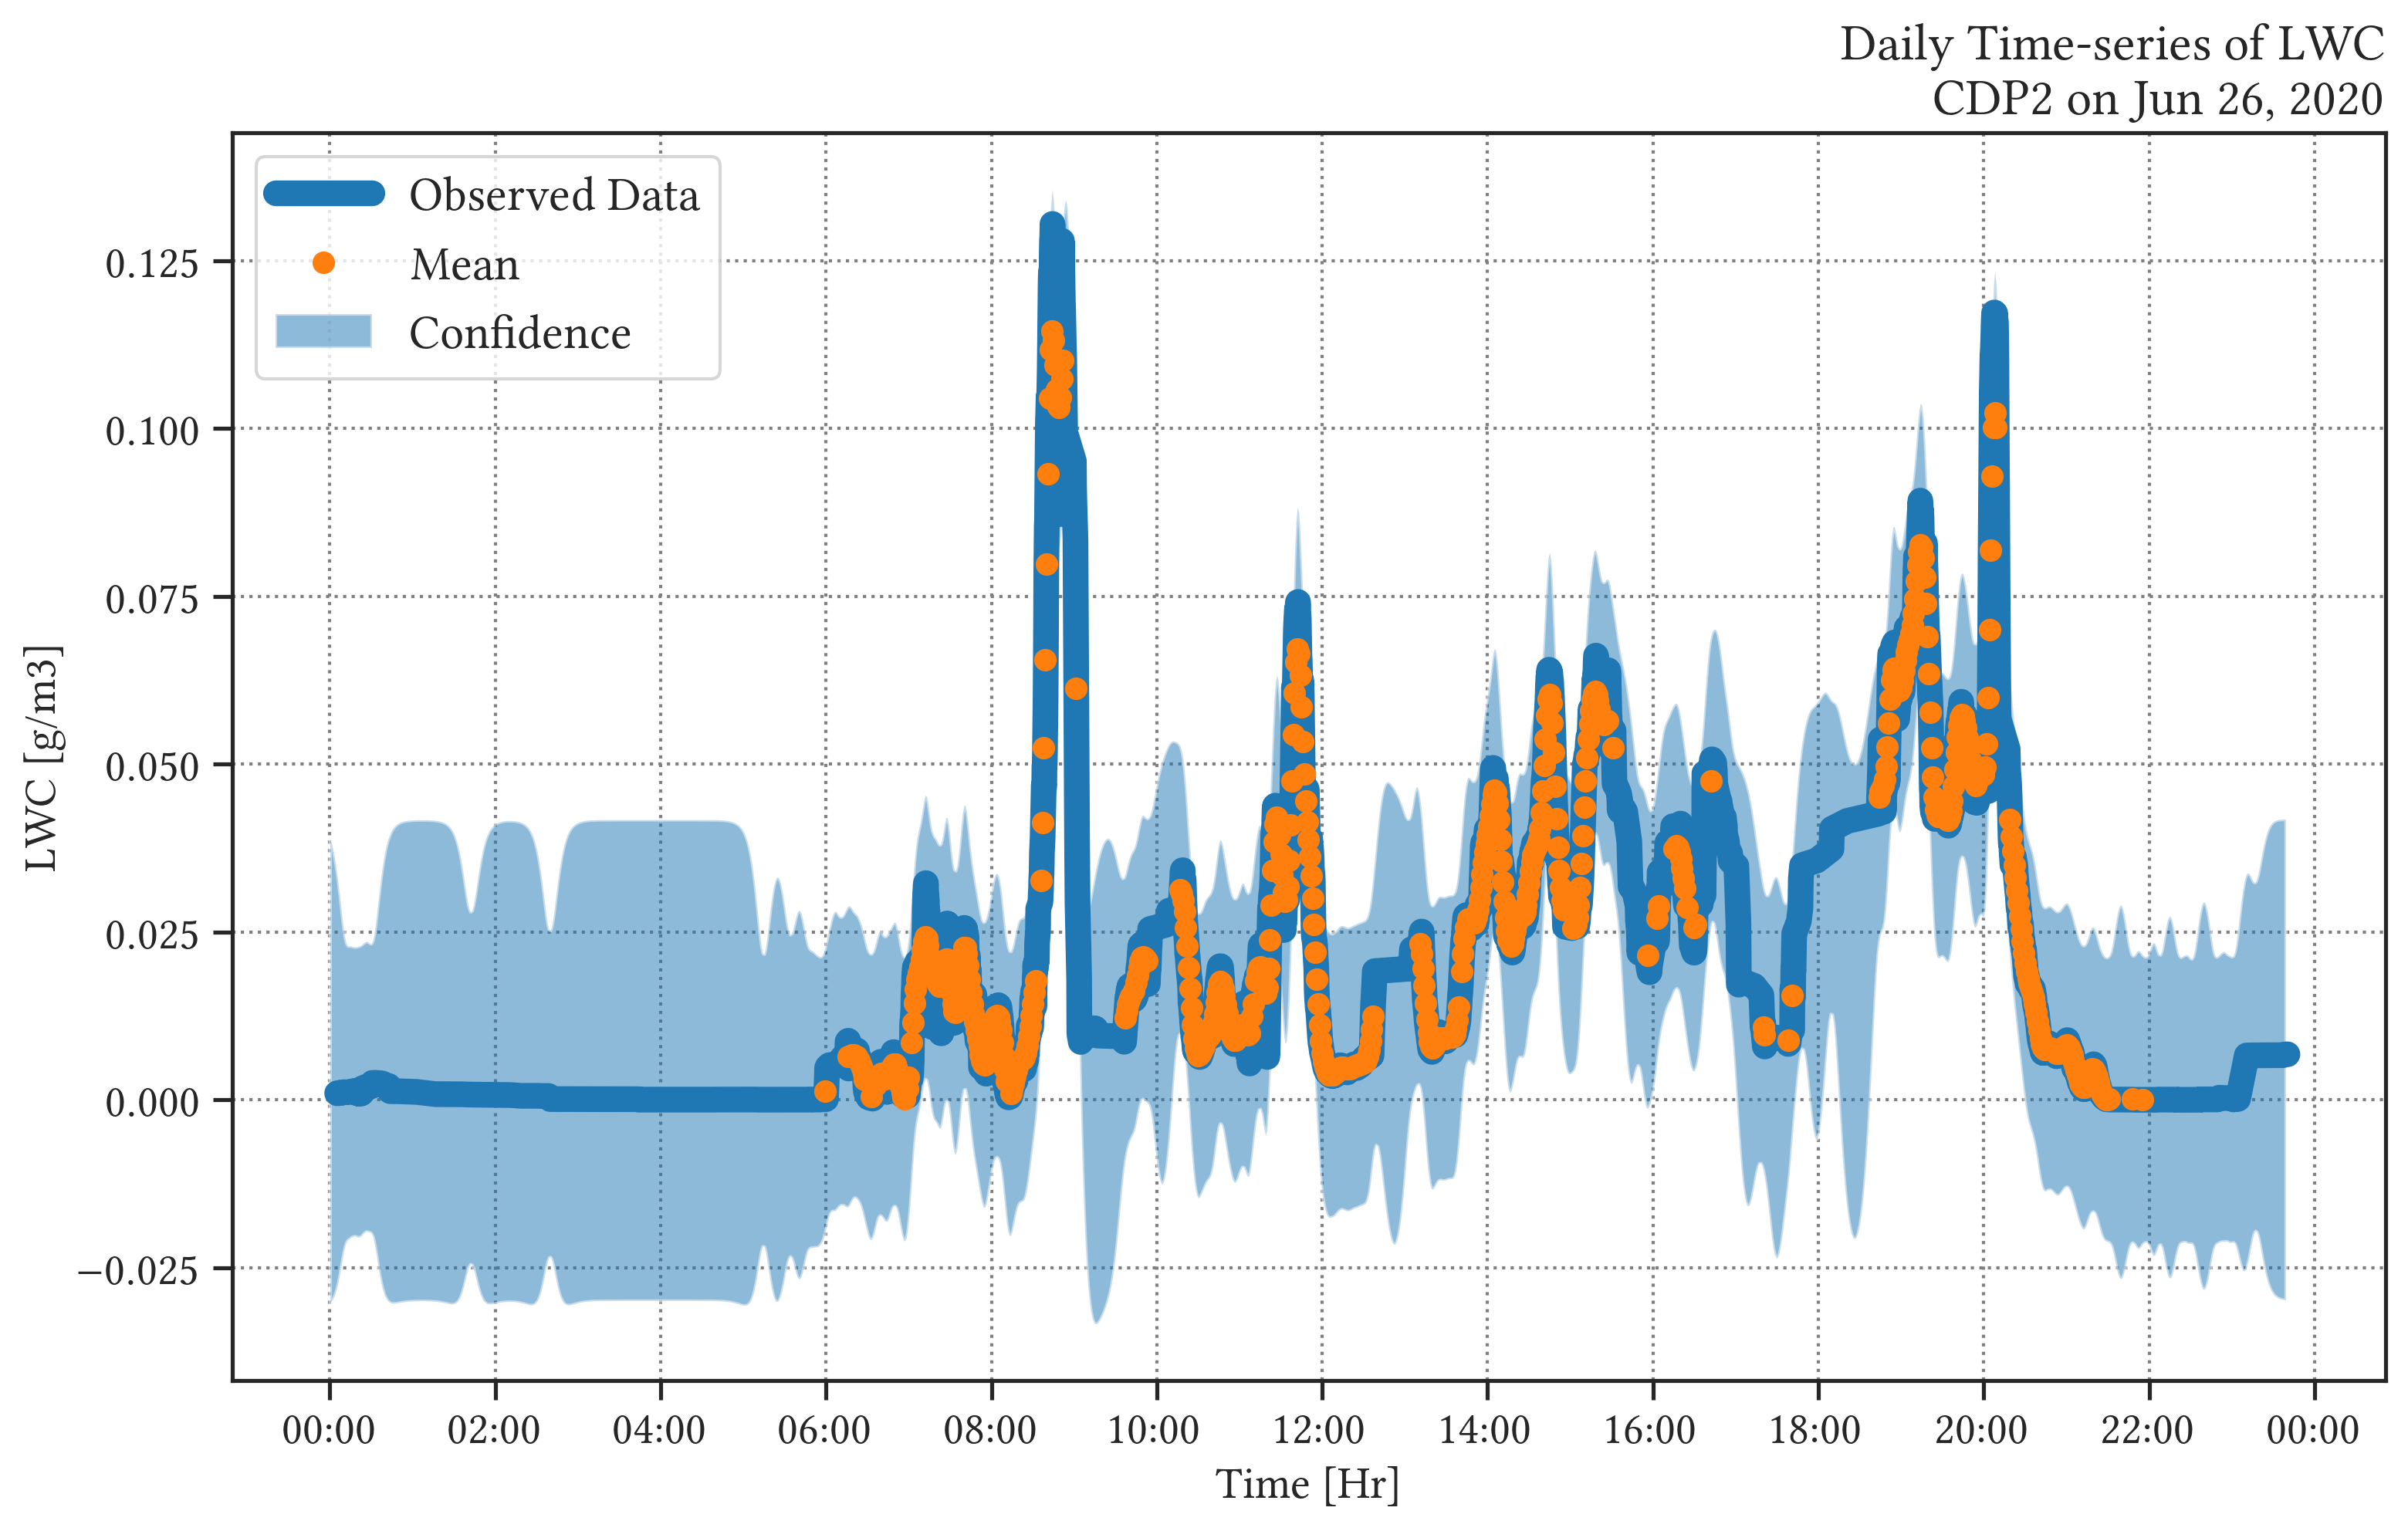
\includegraphics[width=0.7\textwidth]{img/sgp.png}
        \caption{Daily time-series of LWC [g/m$^3$] on June 26th, 2020}
    \end{figure}
\end{frame}

\end{document}